\chapter{The~wavelets}\label{chap:wavelets_comp}

This chapter consists of two sections. In the~first one (\ref{sec:wavelets}), we will briefly and formally describe the~main principle and usage of second generation wavelet transformation methods which are relevant for this thesis. In the~second one (\ref{sec:wavelets_cbdam}), we will compare C-BDAM and our method to these methods. Even though C-BDAM is based on the~same principle, it differs from these methods a~bit, so we will describe the basic differences. Then we will perform the~same basic comparison with our proposed method. Our method differs from the~described wavelet scheme and C-BDAM a~bit more which will be clarified in that section.

\section{The~introduction to second-generation wavelets}\label{sec:wavelets}
Basically, there are two generations of wavelets. The~first generation uses dilated and translated wavelet function~\cite{waveletsTutorial} for computation. The~second one uses filter banks to perform high-pass and low-pass filtering~\cite{waveletsLifting}. The~computational equivalency of these two approaches has been proven~\cite{waveletsEquiv}.

For this work, the~second generation of discrete wavelet transform methods is most relevant, so we will briefly describe it in this section in order to give the~reader an~idea of the~wavelet concept which is referred to in many places of this thesis. The~second wavelet generation is much easier to understand than the~first one, so it is possible to describe its basic idea in a~few pages.

Every method of this generation consists of just several subsequent applications of lifting onto the~input. The~lifting is the~basic step of the~method. It splits the~set of its input signal samples into two parts - low-pass (the~low frequency information) and high-pass (residuals, the~high frequency information). The~lifting is firstly applied on the~input set of signal samples and then is recursively applied to the~low-pass part produced in the~previous iteration until the~length of the~latest low-pass part is 1. In order to make this recursion possible, the~count of samples of the~original input of the~method must be a~certain power of two. If the~length of the input is $2^n$, the~method performs $n$ iterations of lifting. The~described successive application of lifting on smaller and smaller input is called the~bottom-top pass. We can imagine this as building a~pyramid of low-pass outputs the~first tier of which is the~input itself and every following higher tier is the~low-pass output of lifting applied to the~tier right below. Every tier is half the~width of the~previous one and after the~bottom-top pass, the~highest tier has the~width of 1.

After this bottom-top pass, we can perform the~inverse top-bottom pass. This pass does not know how the~produced pyramid looks, it only knows its highest tier, sized 1. However, it is supposed to be able to progressively reconstruct the~whole pyramid from the~top to the~bottom, only utilizing the~knowledge of the~high-pass information. Producing a~certain tier from the~previos one is called the~reconstruction which is the~exact opposite of lifting.

At this point, you might ask what all these decompositions and backward compositions are good for. What makes them interesting is the~fact that the~bottom-top pass just needs the~high-pass information (residuals) to fully reconstruct the~input. This information tends to be sparse and input-dependent - the~smoother the~input, the~less high-pass information it contains. If we compress it well, we can save much storage space. Thus, if we want to store a~set of samples the~count of which is a~power of two in as little space as possible, we will not store the~samples directly, but we will store just the~compressed residuals produced by the~successive iterations of lifting applied to the~input. If we are not required to accurately reconstruct the~input, we can even decimate (quantize) the~residuals. Because this information often contains just details, its careful decimation does not deform the~reconstruction much and ensures better compression ratio. One more interesting fact is that the~residuals bound to lower tiers of the~pyramid carry finer details than those bound to the~higher ones. Thanks to this, the~more-detailed (larger) sets of residuals can be compressed more aggressively than the~less-detailed (smaller) ones. This is called progressive compression and it is used for example in JPEG standard~\cite{jpeg}.

In the~following lines, we will describe the~lifting and reconstruction steps more formally.
Let us say that the~lifting is given the~input samples $x_k$. It splits them into the~even ones:~$x_{2k} = x_e$ and the~odd ones:~$x_{2k+1} = x_o$. This splitting is not yet based on any frequency properties of the~samples, it is based just on their order. However, these two sets of samples will subsequently be modified, so that the~even ones will contain the~low-pass information and the~odd ones will become the~residuals - the~high-pass information. This will be performed with the~help of two operators: the~prediction operator $P$ and the~update operator $U$. $P$ will be used to produce the~residuals $d$ from $x_o$ and $U$ will be used to produce the~low-pass part $s$ from $x_e$.

Up to this point, just the~common properties of the~second-generation methods have been described. Now will come the~differences between them. The only thing they differ in is the~way they perform lifting and reconstruction. The way the~lifting step is performed clearly determines the~way how the~reconstruction is performed, as the~reconstruction must be the~exact inverse of lifting. The~lifting step varies in the~order in which the~operators $P$ and $U$ are applied. According to this, the~methods can be split into two main groups - the~prediction-first ones and the~update-first ones.

In the~prediction-first methods, the~prediction is applied first:

$$d = x_o - P(x_e)$$
$$s = x_e + U(d)$$

The~reconstruction must be the~exact inverse:

$$x_e = s - U(d)$$
$$x_o = d + P(x_e)$$

In the~update-first methods, the~update operator is applied first:

$$s = x_e + U(x_o)$$
$$d = x_o - P(s)$$

Here is how the~reconstruction looks then:

$$x_o = d + P(s)$$
$$x_e = s - U(x_o)$$

\section{Comparisons between the~wavelets, C-BDAM and our method}\label{sec:wavelets_cbdam}
In this section, we will describe how C-BDAM and our method differ from the~basic second-generation wavelet scheme and from each other. The~lifting inside C-BDAM is a~slight variation of the~update-first approach. The~main difference is that the~input to the~first update is not only $x_o$, but the~whole $x$. In addition, the~computation of $s$ is not the~summation of the~product of $x_e$ and $U$ anymore, because inside $U(x)$, $x_e$ is multiplied:

$$s = U(x)$$
$$d = x_o - P(s)$$

The~inverse reconstruction is then:

$$x_o = d + P(s)$$
$$x_e = U^{-1}(x)$$

Moreover, the~samples $x$ are regularly distributed in the~plane, so the~spliting into $x_o$ and $x_e$ no longer depends on the~indices of the~samples, but on their positions instead~(Fig.~\ref{fig:cbdam_lifting}). Nevertheless, this is just a~formal difference which has no effect on the~computation. The~size of $x_o$ and $x_e$ is still half the~size of $x$ which is crucial to keep the~original form of lifting. Note that if the~residuals $d$ were simply quantized after lifting and used in the~reconstructions inside the~second top-bottom pass, each step of the~reconstruction would increase the~maximum absolute deviation from the~original low-pass values produced on the~first bottom-top pass. To ensure that the~reconstructed values are within the~maximum-error bound from their corresponding values produced in the~first pass at each tier, the~residuals computed in the~first pass are slightly corrected according to the~actual values in another additional top-bottom pass which then turns out to be identical to the~reconstruction (decompression), except for the~fact that in the~following decompression, just the~corrected residuals are used to progressively reconstruct the~data.

\newcommand*{\captionsource}[2]{%
	\caption[{#1}]{%
		#1%
		\\\hspace{\linewidth}%
		\textbf{Source:} #2%
	}%
}

\begin{figure}
	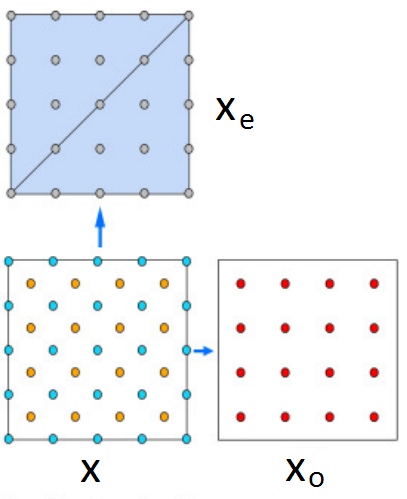
\includegraphics[width=0.28\textwidth]{figures/cbdam_lifting.png}\centering
	\captionsource{Lifting in C-BDAM - the~samples $x$ are split into the~even ones ($x_e$) which will become low-pass ($s$) and the~odd ones ($x_o$) which will become high-pass ($d$)}{C-BDAM~\cite{cbdam} (edited)}
	\label{fig:cbdam_lifting}
\end{figure}

The~method proposed in this thesis shares the~same main lifting principle with C-BDAM - it is update-first and uses the~whole $x$ as the~input to $U$, but has several differences: the~size of $x_e$ and thus $s$ is not half the~size of $x$, but one fourth of it instead, as each four neighboring pixels of $x$ are collapsed into one inside $s$~(Fig.~\ref{fig:subst}). Additionally, the~lifting is not complete, because the~prediction operator is not applied there and the~computation of residuals is not performed there either. In the~lifting of C-BDAM, just temporary approximate residuals are computed and they are corrected in the~subsequent top-bottom pass, whereas in our method, the~correct residuals which already ensure the~satisfaction of the~maximum-error bound constraint are computed directly in the~second top-bottom pass, also utilizing the~prediction operator. Similarly to C-BDAM, the~computations inside this pass are identical to the~reconstruction of the~data, except for the~fact that during the~reconstruction, the~residuals are not computed anymore. Additionally, the~prediction operator is applied multiple times in one step of the~reconstruction which is explained in Chapter~\ref{chap:details}. The~rationale behind these differences is explained in Chapter.~\ref{chap:cbdam_comp}.
